\documentclass[../psets.tex]{subfiles}

\pagestyle{main}
\renewcommand{\leftmark}{Problem Set \thesection}
\setcounter{section}{4}
\setenumerate[1]{label={\textbf{\arabic*.}}}
\setenumerate[2]{label={(\arabic*)}}

\begin{document}




\section{Fixed Points and Perturbation}
\subsection*{Problems Related to Fundamental Definitions}
\begin{enumerate}
    \item \marginnote{11/10:}Are the following real functions Lipschitz continuous near 0? If yes, find a Lipschitz constant for some interval containing 0.
    \begin{enumerate}
        \item $1/(1-x^2)$.
        \begin{proof}
            \fbox{Yes.} Consider the interval $[-0.5,0.5]$. Then we may take
            \begin{equation*}
                \boxed{L = \frac{16}{9}}
            \end{equation*}
        \end{proof}
        \item $x\log|x|$.
        \begin{proof}
            \fbox{No.}
        \end{proof}
        \item $x^2\sin(1/x)$.
        \begin{proof}
            If we take the piecewise function consisting of the above expression on $\R\setminus\{0\}$ and 0 at 0, then \fbox{yes.} Consider the interval $[-1,1]$. Then we may take
            \begin{equation*}
                \boxed{L = 2}
            \end{equation*}
        \end{proof}
    \end{enumerate}
    \item Find the first two elements $y_1(t),y_2(t)$ for the Picard iteration sequence of the following initial value problems, and estimate the error between $y_2(t)$ and the actual solution. Since they are all of separable form, the actual solutions can be explicitly found.
    \begin{enumerate}
        \item $y'=1+y^2$, $y(0)=0$.
        \begin{proof}
            We take $y_0(t)=0$. Then
            \begin{align*}
                y_1(t) &= y_0(0)+\int_0^t[1+y_0(t)^2]\dd{t}\\
                &= \int_0^t[1+0]\dd{t}\\
                \Aboxed{y_1(t) &= t}
            \end{align*}
            and
            \begin{align*}
                y_2(t) &= y_0(0)+\int_0^t[1+y_1(t)^2]\dd{t}\\
                &= \int_0^t[1+t^2]\dd{t}\\
                \Aboxed{y_2(t) &= t+\frac{t^3}{3}}
            \end{align*}
            The error is between $y_2$ and the actual solution $y(t)=\tan(t)$ is given by
            \begin{equation*}
                \boxed{\varepsilon = \tan(t)-t-\frac{t^3}{3}}
            \end{equation*}
        \end{proof}
        \item $y'=2ty$, $y(0)=1$.
        \begin{proof}
            We take $y_0(t)=1$. Then
            \begin{align*}
                y_1(t) &= y_0(0)+\int_0^t2ty_0(t)\dd{t}\\
                &= 1+\int_0^t2t\dd{t}\\
                \Aboxed{y_1(t) &= 1+t^2}
            \end{align*}
            and
            \begin{align*}
                y_2(t) &= y_0(0)+\int_0^t2ty_1(t)\dd{t}\\
                &= 1+\int_0^t[2t+2t^3]\dd{t}\\
                \Aboxed{y_2(t) &= 1+t^2+\frac{t^4}{2}}
            \end{align*}
            The error is between $y_2$ and the actual solution $y(t)=\e[t^2]$ is given by
            \begin{equation*}
                \boxed{\varepsilon = \e[t^2]-1-t^2-\frac{t^4}{2}}
            \end{equation*}
        \end{proof}
        \item $y'=y/(1-t)$, $y(0)=1$.
        \begin{proof}
            We take $y_0(t)=1$. Then
            \begin{align*}
                y_1(t) &= y_0(0)+\int_0^t\frac{y_0(t)}{1-t}\dd{t}\\
                &= 1+\int_0^t\frac{1}{1-t}\dd{t}\\
                \Aboxed{y_1(t) &= 1-\ln|1-t|}
            \end{align*}
            and
            \begin{align*}
                y_2(t) &= y_0(0)+\int_0^t\frac{y_1(t)}{1-t}\dd{t}\\
                &= 1+\int_0^t\frac{1-\ln|1-t|}{1-t}\dd{t}\\
                \Aboxed{y_2(t) &= 1-\ln|1-t|+\frac{1}{2}(\ln|1-t|)^2}
            \end{align*}
            The error between $y_2$ and the actual solution $y(t)=\e[-\ln|1-t|]$ is given by
            \begin{equation*}
                \boxed{\varepsilon = \e[-\ln|1-t|]-1+\ln|1-t|-\frac{1}{2}(\ln|1-t|)^2}
            \end{equation*}
        \end{proof}
    \end{enumerate}
    \pagebreak
    \item Check whether the implicit equation $F(x,y)=0$ uniquely determines an explicit function $y=f(x)$ around the given point $(x_0,y_0)$. If it does, compute $f'(x_0)$.
    \begin{enumerate}
        \item For $(x,y)\in\R^2$, $F(x,y)=x^2+y^2-1$, $(x_0,y_0)=(\sqrt{2}/2,-\sqrt{2}/2)$.
        \begin{proof}
            From the implicit equation, we have that
            \begin{align*}
                0 &= x^2+y^2-1\\
                y &= \pm\sqrt{1-x^2}
            \end{align*}
            Since
            \begin{align*}
                -\frac{\sqrt{2}}{2} &= -\sqrt{1-\left( \frac{\sqrt{2}}{2} \right)^2}\\
                y_0 &= -\sqrt{1-x_0^2}
            \end{align*}
            our explicit function \fbox{is uniquely determined around $(x_0,y_0)$.}\par
            Moreover, we can compute that
            \begin{align*}
                f'(x_0) &= \frac{2x_0}{2\sqrt{1-x_0^2}}\\
                \Aboxed{f'(x_0) &= 1}
            \end{align*}
        \end{proof}
        \item For $(x,y)\in\R^2$, $F(x,y)=x^2-y^2-1$, $(x_0,y_0)=(1,0)$.
        \begin{proof}
            From the implicit equation, we have that
            \begin{align*}
                0 &= x^2-y^2-1\\
                y &= \pm\sqrt{x^2-1}
            \end{align*}
            Since
            \begin{align*}
                y_0 &= \sqrt{x_0^2-1}&
                y_0 &= -\sqrt{x_0^2-1}
            \end{align*}
            our explicit function \fbox{is not uniquely determined around $(x_0,y_0)$.}
        \end{proof}
        \item For $(x,y)\in\R^2$, $F(x,y)=x\e[y]+y$, $(x_0,y_0)=(0,0)$.
        \begin{proof}
            We apply the implicit function theorem.\par\smallskip
            $F$ is defined on a subset of $\R^2$, as desired.\par
            We have that
            \begin{align*}
                \pdv{F}{x} &= \e[y]&
                \pdv{F}{y} &= x\e[y]+1
            \end{align*}
            Since both of the above partial derivatives are continuous, $F$ is continuously differentiable on its domain, as desired.\par
            $(x_0,y_0)=(0,0)\in\R^2$, which is the domain of $F$, as desired.\par
            $F(x_0,y_0)=0\e[0]+0=0$, as desired.\par
            The truncated Jacobian matrix is $1\times 1$ and contains a nonzero element at $(x_0,y_0)$ --- in particular, it contains $\pdv*{F}{x}$ --- as desired.\par\smallskip
            Therefore, our explicit function \fbox{is uniquely determined around $(x_0,y_0)$.}\par\smallskip
            Moreover, we can compute that
            \begin{align*}
                f'(x_0) &= -\left( \pdv{F}{y}(x_0,y_0) \right)^{-1}\cdot\pdv{F}{x}(x_0,y_0)\\
                &= -\left( 0\e[0]+1 \right)^{-1}\cdot\e[0]\\
                \Aboxed{f'(x_0) &= -1}
            \end{align*}
        \end{proof}
    \end{enumerate}
\end{enumerate}


\subsection*{Problems Involving the Banach Fixed Point Theorem}
\begin{enumerate}
    \item 
    \begin{enumerate}
        \item Show that the condition "constant $q<1$" in the statement of the Banach fixed point theorem is not redundant. You may give an example of a function $f:\R\to\R$ which satisfies the strict inequality $|f(x)-f(y)|<|x-y|$ but does not have a fixed point.
        \begin{proof}
            Choose
            \begin{equation*}
                \boxed{
                    f(x) =
                    \begin{cases}
                        1 & x\leq 0\\
                        x+\e[-x] & x>0
                    \end{cases}
                }
            \end{equation*}
            The fact that
            \begin{equation*}
                \dv{f}{x} =
                \begin{cases}
                    0 & x\leq 0\\
                    1-\e[-x] & x>0
                \end{cases}
            \end{equation*}
            implies that $|\dv*{f}{x}|<1$ for all $x$. Hence, $f$ satisfies the desired strict inequality. Additionally, since the graph of $f(x)>x$ for all $x$ (as can be readily verified from its definition), it has no fixed point, as desired.
        \end{proof}
        \item Let $f:\R^n\to\R^n$ be a Lipschitz mapping with uniform Lipschitz constant $q<1$, that is,
        \begin{equation*}
            |f(x)-f(y)| \leq q|x-y|
        \end{equation*}
        for all $x,y\in\R^n$. Prove that the mapping $x\mapsto x+f(x)$ is invertible with Lipschitz continuous inverse.
        \begin{proof}
            % WTS: There exists $x\in\R^n$ such that $y=g(x)=x+f(x)$.
            % $f$ has a unique fixed point $x\in\R^n$.

            % it is injective and surjective.\par
            % Injectivity: Suppose $g(x)=g(y)$. Then
            % \begin{align*}
            %     x+f(x) &= y+f(y)\\
            %     f(x)-f(y) &= y-x\\
            %     |f(x)-f(y)| &= |x-y|
            % \end{align*}
            % It follows by substituting into the Lipschitz condition that
            % \begin{equation*}
            %     |x-y| \leq q|x-y|
            % \end{equation*}
            % This combined with the fact that
            % \begin{align*}
            %     q &< 1\\
            %     q|x-y| &\leq |x-y|
            % \end{align*}
            % proves that
            % \begin{align*}
            %     |x-y| &= q|x-y|\\
            %     (1-q)|x-y| &= 0\\
            %     |x-y| &= 0\\
            %     x &= y
            % \end{align*}
            % as desired.\par

            % We have that
            % \begin{align*}
            %     |g(x)-g(y)| &= |[x+f(x)]-[y+f(y)]|\\
            %     &= |[x-y]+[f(x)-f(y)]|\\
            %     &\leq |x-y|+|f(x)-f(y)|\\
            %     &\leq |x-y|+q|x-y|\\
            %     &= (1+q)|x-y|
            % \end{align*}
            % Let $x,y\in\R^n$ be arbitrary. Then
            % \begin{align*}
            %     |g^{-1}(x)-g^{-1}(y)| &= |a-b|
            % \end{align*}
            
            % WTS: $|g^{-1}(x)-g^{-1}(y)|\leq|x-y|$.

            % WTS: $|x-y|\leq|g(x)-g(y)|$.
            % To prove that $g^{-1}$ is Lipschitz continuous, it will suffice to show that
            % \begin{equation*}
            %     |g^{-1}(x)-g^{-1}(y)| \leq |x-y|
            % \end{equation*}
            % for all $x,y\in\R^n$. Let $x,y\in\R^n$ be arbitrary. Then
            % \begin{align*}
            %     |g^{-1}(x)-g^{-1}(y)| &= |
            % \end{align*}
            % \begin{align*}
            %     |g(x)-g(y)| &= |x-y+f(x)-f(y)|\\
            %     &\leq |x-y|+|f(x)-f(y)|\\
            %     &\geq |x-y|
            % \end{align*}


            Let $g:\R^n\to\R^n$ be defined by $g(x)=x+f(x)$. To prove that $g$ is invertible, it will suffice to show that $g$ is one-to-one, that is, for every $b\in\R^n$, there exists a unique $a\in\R^n$ such that $g(a)=b$. Let $b\in\R^n$ be arbitrary. Define $h:\R^n\to\R^n$ by $h(x)=b-f(x)$. Then since
            \begin{align*}
                |h(x)-h(y)| &= |[b-f(x)]-[b-f(y)]|\\
                &= |f(y)-f(x)|\\
                &= |f(x)-f(y)|\\
                &\leq q|x-y|
            \end{align*}
            we have by the Banach fixed point theorem that there exists a unique $a\in\R^n$ such that $a=h(a)$. It follows that
            \begin{align*}
                a &= b-f(a)\\
                a+f(a) &= b\\
                g(a) &= b
            \end{align*}
            as desired.\par
            To prove that $g^{-1}$ is Lipschitz continuous, it will suffice to show that
            \begin{equation*}
                |g^{-1}(x)-g^{-1}(y)| \leq \frac{1}{1-q}|x-y|
            \end{equation*}
            for all $x,y\in\R^n$. Let $x,y\in\R^n$ be arbitrary. Define $a=g^{-1}(x)$ and $b=g^{-1}(y)$. Then since the first term below is nonnegative (as the product of two nonnegative numbers), we have that
            \begin{align*}
                (1-q)|a-b| &= |a-b|-q|a-b|\\
                &\leq |a-b|-|f(a)-f(b)|\\
                &= |a-b|-|f(b)-f(a)|\\
                &= \big| |a-b|-|f(b)-f(a)| \big|\\
                &\leq |[a-b]-[f(b)-f(a)]|\\
                &= |[a+f(a)]-[b+f(b)]|\\
                &= |g(a)-g(b)|
            \end{align*}
            It follows by returning the substitution that
            \begin{align*}
                (1-q)|g^{-1}(x)-g^{-1}(y)| &\leq |x-y|\\
                |g^{-1}(x)-g^{-1}(y)| &\leq \frac{1}{1-q}|x-y|
            \end{align*}
            as desired.
        \end{proof}
    \end{enumerate}
    \item Consider the following iterative algorithm to compute the square root of a given $a>1$.
    \begin{equation*}
        x_{n+1} = \frac{1}{2}\left( x_n+\frac{a}{x_n} \right)
    \end{equation*}
    \begin{enumerate}
        \item Show that the function
        \begin{equation*}
            F(x) = \frac{1}{2}\left( x+\frac{a}{x} \right)
        \end{equation*}
        meets the requirements of the contraction mapping principle on the closed interval $[\sqrt{a/2},a]$. Prove that $x_n\to\sqrt{a}$.
        \begin{proof}
            We want to show that
            \begin{equation*}
                |F(x)-F(y)| \leq q|x-y|
            \end{equation*}
            for some $q\in(0,1)$ and all $x,y\in[\sqrt{a/2},a]$.

            We have that
            \begin{align*}
                |F(x)-F(y)| &= \left| \frac{1}{2}\left( x+\frac{a}{x} \right)-\frac{1}{2}\left( y+\frac{a}{y} \right) \right|\\
                &= \frac{1}{2}\left| (x-y)+\left( \frac{a}{x}-\frac{a}{y} \right) \right|\\
                &= \frac{1}{2}\left| (x-y)+a\cdot\frac{y-x}{xy} \right|\\
                &= \frac{1}{2}\left| \left( 1-\frac{a}{xy} \right)(x-y) \right|\\
                &= \frac{1}{2}\left| 1-\frac{a}{xy} \right||x-y|\\
                % &\leq \frac{1}{2}|x-y|
            \end{align*}
        \end{proof}
        \item For $a=2$, start the iteration $x_{n+1}=F(x_n)$ with $x_0=1$. Use a calculator to compute the first 10 values of this iteration, up to 11 digits after the decimal point. Compare it with the exponentially converging sequence $1.4,1.41,1.414,1.4142,\dots$. Which of the two algorithms is better?
        \begin{proof}
            We have that
            \begin{empheq}[box=\fbox]{align*}
                x_0 &= 1\\
                x_1 &= 1.5\\
                x_2 &= 1.41666666667\\
                x_3 &= 1.41421568627\\
                x_4 &= 1.41421356237\\
                x_5 &= 1.41421356237\\
                x_6 &= 1.41421356237\\
                x_7 &= 1.41421356237\\
                x_8 &= 1.41421356237\\
                x_9 &= 1.41421356237\\
                x_{10} &= 1.41421356237
            \end{empheq}
            \fbox{The algorithm from part (1) is better.}
        \end{proof}
        \item Try to estimate the error $|x_n-\sqrt{a}|$ as well as possible. \emph{Hint}. There should be something related to an iterative sequence $\{b_n\}$ satisfying
        \begin{equation*}
            b_{n+1} \leq Mb_n^2
        \end{equation*}
        You should prove that the sequence converges to zero faster than any geometric progression.\par
        Context: This algorithm is referred to as \textbf{Newton's method}. It is a rapidly converging algorithm to find zeros/fixed points of functions, capable of giving very precise approximations within very few steps. A variation of it, called the \textbf{Nash-Moser technique}, is a very powerful tool for proving the existence of solutions to nonlinear differential equations.
    \end{enumerate}
    \item In this question, we aim to prove that a certain differential equation admits a unique periodic solution. Let $f(t)$ be a smooth, real-valued function of period 1, that is, $f(t+1)\equiv f(t)$.
    \begin{enumerate}
        \item Fix $a>0$. Prove that there exists only one $x\in\R$ such that the solution of the initial value problem
        \begin{equation*}
            y'+ay = f(t)
            ,\quad
            y(0) = x
        \end{equation*}
        has period 1, and express $x$ in terms of the integral of $f$.
        \item Now let $g(w)$ be some smooth function such that $g'(0)=0$. Prove the following nonlinear perturbative result: For any period 1 continuous function $f$ close to 0, there is only one $x\in\R$ with small magnitude such that the solution of the perturbed initial value problem
        \begin{equation*}
            y'+ay+g(y) = f(t)
            ,\quad
            y(0) = x
        \end{equation*}
        has period 1. \emph{Hint}: Write the solution as $y(t;x)$ and consider the function $x\to y(1;x)$. Try to apply the continuous dependence result discussed in class to conclude that this function is a contraction near $0\in\R$.
    \end{enumerate}
\end{enumerate}


\subsection*{Problems Related to the Calculation of Perturbation}
\begin{enumerate}
    \item Determine the approximate solution of the following initial value problems up to order $\mu$, where $\mu$ is the small perturbative parameter.
    \begin{enumerate}
        \item 
        \begin{equation*}
            y''+(1+\mu)y = 0
            ,\quad
            y(0) = a
            ,\quad
            y'(0) = b
        \end{equation*}
        This is in fact the harmonic oscillator equation. Compare your result with the actual solution, and estimate the time beyond which the approximate solution fails to match it well.
        \item 
        \begin{equation*}
            y' = ry-\mu y^2
            ,\quad
            y(0) = a
        \end{equation*}
        This is in fact the logistic growing model with $\mu=r/M\ll 1$, $M$ being the capacity. Compare your result with the actual solution of the logistic differential equation, and estimate the time beyond which the approximate solution fails to match it well.\par
        It should be stressed again that these approximate solutions only work for a fixed time interval, and usually fail to approximate the actual solution well for large $t$.
    \end{enumerate}
    \item Let $h$ be a small real number. Consider the function
    \begin{equation*}
        f(x) = \cos x+hx\sin x
    \end{equation*}
    We know that when $h=0$, the point $x=2\pi$ is a maximum point of $f(x)$. If $h\neq 0$, the extrema of $f$ cannot be explicitly determined. However, determine the first positive maximum point $x_1(h)$ of $f$ as a function of $h$, up to order $h$. \emph{Hint}: $x_1(h)$ is the zero of $f'(x)$ with $x_1(0)=2\pi$, and you may apply the implicit function theorem.
    \item Let $A,B>0$ be fixed constants, $\mu$ be a real number of small magnitude compared to $A,B$. Determine the approximate solution of the following differential equation up to order $\mu$.
    \begin{equation*}
        \dv[2]{u}{\varphi}+u = A+\mu u^2
        ,\quad
        u(0) = A+B
        ,\quad
        u'(0) = 0
    \end{equation*}
    \emph{Hint}: For the zeroth order approximation, the solution can be easily guessed without using the Duhamel formula.
\end{enumerate}


\subsection*{Bonus Problem}
We have already determined that the orbits of the two-body problem under Newtonian gravity are conic sections in the center of mass frame. However, in actual physical situations, there are multiple effects that lead to correction of the orbit. For Mercury, the closest known planet to the Sun, this correction is much easier to observe than with other planets. These effects break the closedness of the ideally elliptic orbit of Mercury, resulting in very slow precession of the perihelion of the orbit (see the picture, which is very much exaggerated).
\begin{center}
    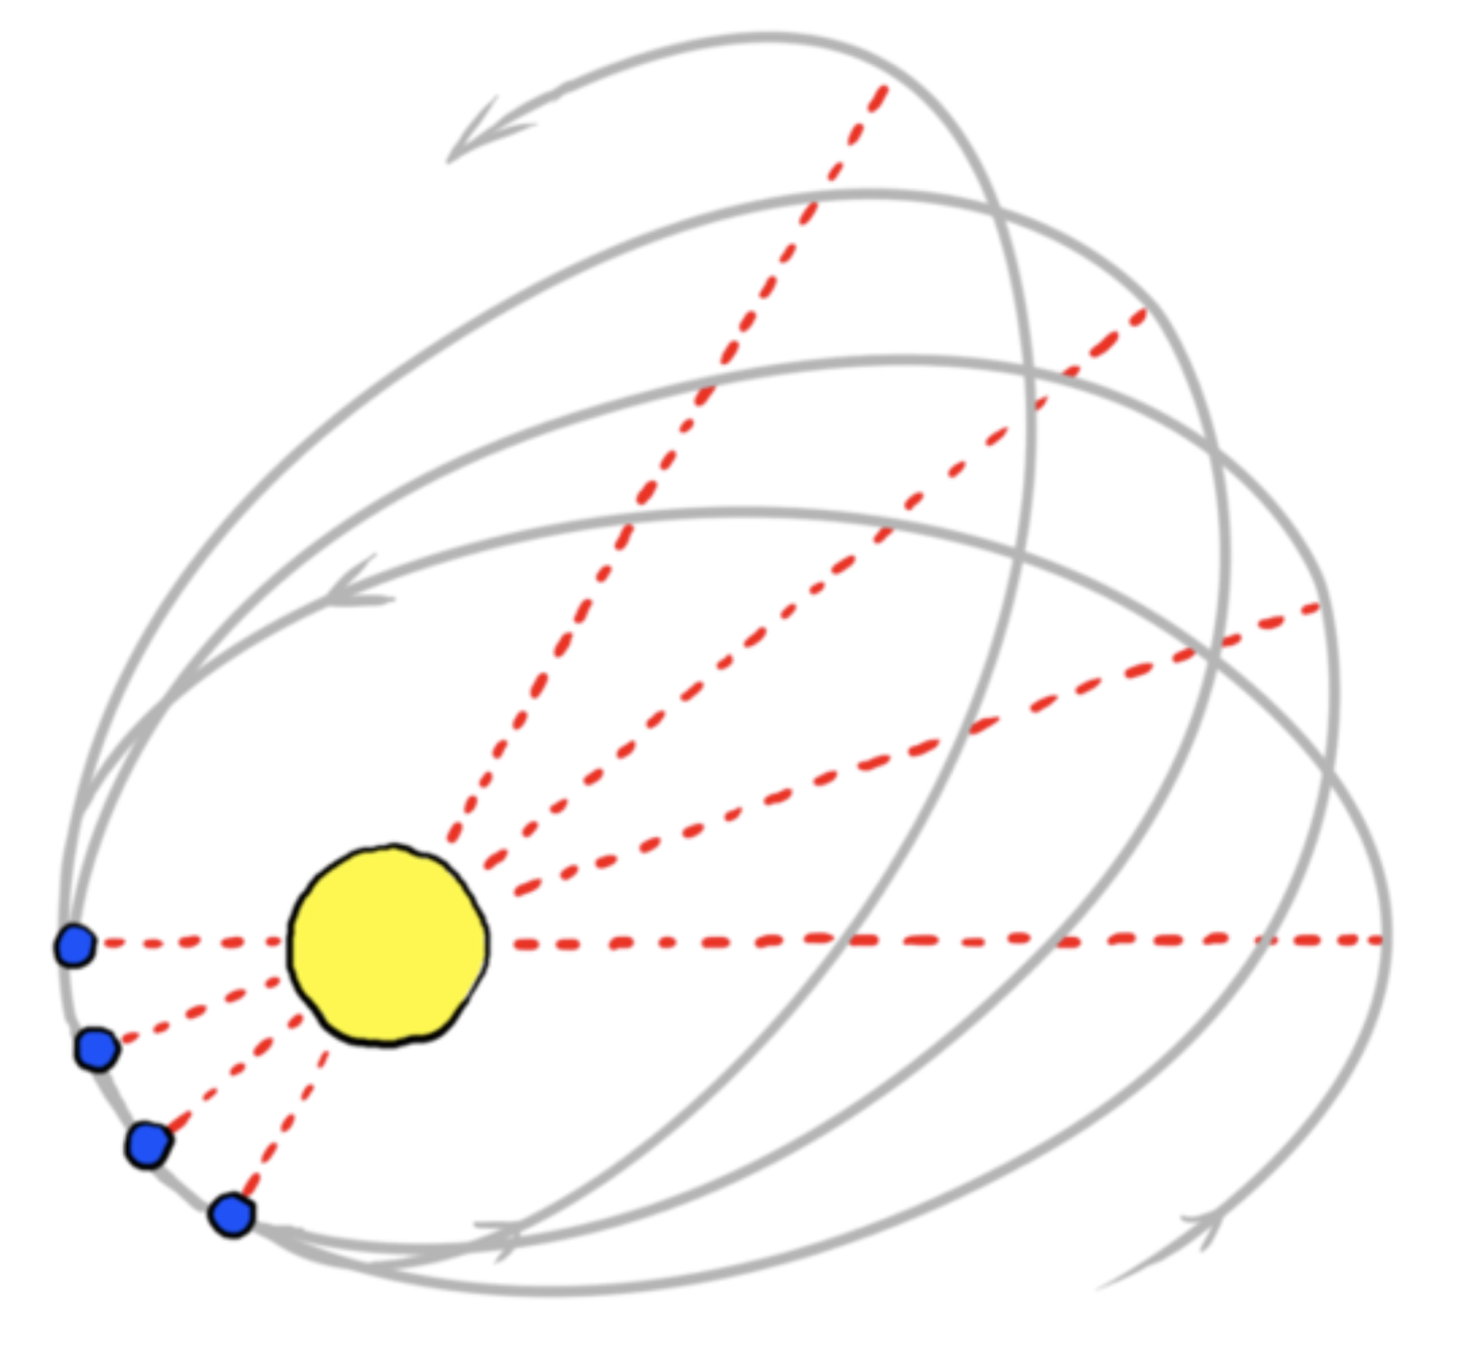
\includegraphics[width=0.4\linewidth]{../ExtFiles/mercuryPrecession.png}
\end{center}
The total observed precession of the perihelion of Mercury is about \num{5600.73} arcsec per century. After deducing the effect of axial precession of the Earth itself, the causes of precession explainable by classical Newtonian gravity theory are shown below.
\begin{center}
    \small
    \renewcommand{\arraystretch}{1.2}
    \begin{tabular}{cc}
        \toprule
        Amount, arcsec per century & Cause\\
        \midrule
        \num{532.3035} & Gravity of other solar bodies\\
        \num{0.0286} & Quadrupole moment of the sun\\
        \num{-0.0020} & Lense-Thirring precession\\
        \num{532.3301} & Total of classical effects\\
        \bottomrule
    \end{tabular}
\end{center}
The observed total after deducing the axial precession of the Earth is, however, \num[separate-uncertainty=true]{574.10\pm 0.65} arcsec per century. There are about 42-43 arcsec per century that cannot be explained by any of the classical effects listed above. This anomalous precession was first observed by Urbain Le Verrier, who assumed that there should be another planet evolving inside the orbit of Mercury. However, his computation did not match with the observation of other planets. Celestial physicists came up with several other assumptions but none of them gave a result consistent with this case. It was only after Albert Einstein's discovery of general relativity that the correction-matching observation was finally obtained. Einstein computed the distortion of Kepler orbits under a special solution, called the \textbf{Schwarzchild solution}, of the relativistic gravitational equation, and his result matches very much for Mercury and for light rays from stars far away in space. These two cases are considered to be the initial powerful experimental supports for general relativity.\par
In this problem, you will be able to reproduce Einstein's result. The physics has been reduced to a minimum and you will find that Einstein's core mathematical argument is a pure perturbative problem for ODEs.\par
In Schwarzchild spacetime, we assume that there is only one static star (the Sun) whose gravitational field is present. The mass of the star is assumed to be $M$, and the spacetime is assumed to be \textbf{spherically symmetric}. The spacetime is parameterized by four coordinates: $t,r,\theta,\varphi$. The $t$ coordinate can be imagined as \emph{time}, and $r,\theta,\varphi$ can be imagined as the spherical coordinates. We describe the "distance" between spacetime points using the Schwarzchild metric
\begin{equation*}
    \dd{s}^2 = -\left( 1-\frac{r_s}{r} \right)c^2\dd{t}^2+\left( 1-\frac{r_s}{r} \right)^{-1}\dd{r}^2+r^2\left( \dd{\theta}^2+\sin^2\theta\dd{\varphi}^2 \right)
\end{equation*}
where $c$ is the speed of light in a vacuum, $G$ is the gravitational constant, and $r_s=2GM/c^2$ is the \textbf{Schwarzchild radius}.\par
The trajectory of a planet in the spacetime is a curve parameterized by the parameter $\tau\in\R$ called the \textbf{proper time of the planet}. The orbit is a \textbf{geodesic} (which is a geometric object, but the definition does not really matter here) in four-dimensional spacetime. Some considerations in symmetry enable us to assume that $\theta\equiv\pi/2$ along the trajectory ("in the ecliptic plane"). Differential geometry guarantees that the spacetime inner product along the orbit should be a constant, i.e.,
\begin{equation}\label{eqn:4.1}
    -c^2 = -\left( 1-\frac{r_s}{r} \right)c^2\left( \dv{t}{\tau} \right)^2+\left( 1-\frac{r_s}{r} \right)^{-1}\left( \dv{r}{\tau} \right)^2+r^2\left( \dv{\varphi}{\tau} \right)^2
\end{equation}
Further considerations in symmetry guarantee that along the trajectory, there are two conserved quantities. These are the relativistic counterparts of total energy and angular momentum.
\begin{align}\label{eqn:4.2}
    \left( 1-\frac{r_s}{r} \right)\dv{t}{\tau} &= \frac{E}{mc^2}&
    mr^2\dv{\varphi}{\tau} &= L
\end{align}
Here, $m$ is the mass of the planet, which is very small compared to $M$.
\begin{enumerate}
    \item We are now interested in the shape of the orbit that we observe as a curve in the ecliptic plane, which can be parameterized as a polar coordinate equation $r=r(\varphi)$. Equations \ref{eqn:4.1}-\ref{eqn:4.2} should imply a differential equation satisfied by $r=r(\varphi)$. Find that differential equation.
    \item Introducing $u=1/r$ and differentiating that equation with respect to $\varphi$ again, you should arrive at an equation of identical form to that of Problem 3.3, i.e., of the form
    \begin{equation*}
        \dv[2]{u}{\varphi}+u = A+\mu u^2
    \end{equation*}
    It can be considered to be a perturbation of the equation presented in HW2 that gives the Kepler orbit. Determine the $A$ and $\mu$ here in terms of the physical constants $G,M,m,c,E,L$. \emph{Hint}: You need to cancel the term $(\dv*{t}{\tau})^2$ in Equation \ref{eqn:4.1} and try to express $(\dv*{r}{\varphi})^2$ in terms of $r$ alone, just as in HW2. This will be the perturbative problem that we are interested in.
    \item Assuming that $\mu$ is small, the equation in the previous problem is a perturbation of the Kepler orbit equation. Thus, it is natural to choose the ray joining the Sun and the perihelion as the polar axis so that we can fix the initial conditions as
    \begin{equation*}
        u(0) = p
        ,\quad
        u'(0) = 0
    \end{equation*}
    where $p$ is the distance from the perihelion to the Sun. The perihelion of the planet corresponds to the maximum of $u$ in the previous problem. Determine the first value of $\varphi$ at which $u$ has a local maximum, up to order $\mu$. Its derivation with $2\pi$ is the \textbf{precession angle}, as the non-periodicity of the solution breaks the closedness of the orbit.\par
    \emph{Hint}: This is in fact Problem 3.2. Your expression should not involve $p$.\par
    Substitute in the following physical constants: $G=\SI{6.673e-11}{\kilo\gram\cubic\meter\per\second\squared}$, $M=\SI{1.989e30}{\kilo\gram}$, $c=\SI{2.998e8}{\meter\per\second}$. Also, the mass of Mercury is $m=\SI{3.301e23}{\kilo\gram}$, the angular momentum of Mercury is $L=\SI{8.983e38}{\kilo\gram\meter\squared\per\second}$, and the revolution period of Mercury is 88 days. Use a calculator to compute the precession angle and convert its unit to arcsec per century (the expression you obtain is, of course, in radians per revolution; also recall that $\SI{1}{arcsec}=\ang{1}/3600$), and compare it with the unexplained precession.
\end{enumerate}




\end{document}